%!TEX program = xelatex
\documentclass[UTF8]{ctexart}
    \usepackage{amsmath}
    \usepackage{geometry}
	\usepackage{graphicx}
	\usepackage[utf8]{inputenc}
	\usepackage{listings}
	\usepackage{url}
    \usepackage{verbatim}
    \usepackage{advdate}
	
	\graphicspath{ {./images/} }

    \title{$LL(1)$语法分析程序说明文档}
    \author{2016211305班 \ 熊光正 (学号:2016211249)}
    \date{\AdvanceDate[-1]\today}
\begin{document}
\lstset{numbers=left,frame=single,breaklines=true}
\maketitle
\tableofcontents
\clearpage
\section{概述}
根据要求,程序输入文法及待分析的句子,输出分析表及分析结果。
即从用户输入或指定的文本文件读取文法四元组,依据算法$4.2$等检查、改造文法,消除空产生式,消除左递归,提前左公因子,
构建$FIRST$集、$FOLLOW$集和预测分析表,依据算法$4.1$等分析输入的句子,并在必要时进行错误处理。
程序假设输入的文法不含环路,但可能包含直接或间接左递归。程序使用迭代使用各算法完成上述目标。
\section{数据结构}
程序使用的数据结构如下:
\begin{table}[!h]
    \centering
    \caption{数据结构表}
    \begin{tabular}{|c|c|c|}
    \hline
    逻辑结构 & 数据结构 & 备注 \\ \hline
    (任意)符号  &  $symbol$ & 即$string$  \\ \hline
    终结符  &  $Terminal$ & 即$symbol$  \\ \hline
    非终结符  & $Nonterminal$  &   \\ \hline
    文法规则 & $Rule$  &   \\ \hline
    非终结符表 & $unordered\_map<symbol, Nonterminal>$  &   \\ \hline
    候选式 & $vector<symbol>$  & 即$Candidate$  \\ \hline
    分析表中的行 & $unordered\_map<Terminal, int>$  & 整数表示对应候选式的序号  \\ \hline
    符号栈 & $vector<Terminal>$  &   \\ \hline
    \end{tabular}
    \end{table}
\section{程序功能}
\subsection{识别文法的形式定义}
程序从字符串识别文法,将其转换成内部表示的非终结符表、终结符表、开始符号和产生式列表。
\subsection{检查并改造文法}
程序检查识别的文法是不是$LL(1)$文法,若不是,则尝试改造文法,即消除空产生式、消除直接和间接左递归、提取公共左因子。
\subsection{构建预测分析表}
程序依次构建$FIRST$集和$FOLLOW$集,并依次建立带同步标记的预测分析表。
\subsection{分析输入的句子}
程序依据上述预测分析表,分析输入的句子,若检测到错误,进行错误处理。
\section{程序运行流程及算法}
\subsection{构建语法}
\subsubsection{输入文法形式定义的词法、语法分析}
程序使用换行符分割输入流中的非终结符、终结符、开始符号和各产生式等参数。对于各参数,程序使用空格分隔其中的各个符号,形成单词符号串。
程序依据文法形式定义的语法处理上述单词符号串,并构建由左部非终结符和右部候选式列表组成的$Rule$语法对象。
程序遍历上述语法对象中的候选式,将其加入内部表示的语法结构。
程序不对此处的分析流程进行错误处理。
\subsubsection{消除空产生式}
为消除左递归,程序需先消除空产生式。程序遍历各非终结符及其各个候选式,
递归从左至右遍历其中的各个符号,若其$FIRST$集中包含空产生式,即为含空产生式的非终结符,
则再递归检查删去该符号后的候选式,将其加入候选式列表。
考虑开始符号,若包含空产生式,则将空产生式加入其候选式列表。
\subsubsection{消除直接和间接左递归}
为构建$LL(1)$分析表,文法需不包含左递归,故程序基于算法$2.1$消除直接和间接左递归。
除开始符号外,程序按字典序升序排列各非终结符,对于除开始符号外的非终结符,程序迭代遍历其的候选式列表,
循环将候选式中的开始符号和排在其前面的非终结符替换为对应的候选式,一次替换一个,若有非终结符被替换,则再循环一次。
接着消除新候选式列表中的直接左递归,并插入新非终结符。若有非终结符被插入,则再遍历一次非终结符列表。
\subsubsection{提取左公因子}
要构建$LL(1)$预测分析表,则文法中的候选式列表不能包含公共左前缀。
程序遍历各非终结符的候选式列表,并构建“首符号-候选式”哈希表,遍历该哈希表,
若存在对应多个候选式的首符号,即该候选式列表中存在公共前缀,则插入新的非终结符。
若有新的非终结符被插入,则重新遍历非终结符列表,直至不再有新的非终结符被插入。
\subsubsection{计算$FIRST$集}
程序迭代遍历非终结符表及其候选式列表,从左至右扫描候选式,
若遇到终结符,将其加入$FIRST$集,并跳出循环,
若遇到非终结符,检查其$FIRST$集,
若其中有空产生式,则继续检查下一个符号,
若不含空产生式,则将其$FIRST$集与当前$FIRST$集合并。
若$FIRST$集有变化,则再遍历一次非终结符列表。
\subsubsection{计算$FOLLOW$集}
程序先将终止符$\$$加入开始符号的$FOLLOW$集,再遍历各非终结符的产生式,
将不在候选式末尾的非终结符后面的字符串的$FIRST$集合并至该非终结符的$FOLLOW$集,
将候选式对应的非终结符的$FOLLOW$集合并至各候选式尾符号的$FOLLOW$集。
若至少一个$FOLLOW$集增大了,则在遍历一次各非终结符的产生式。
\subsubsection{构建带同步记号的预测分析表}
程序基于算法$4.2$构建预测分析表。程序遍历各个非终结符,遍历其候选式列表,计算各个候选式$candidate$的$FIRST$集。
对于其中除空产生式外的元素$word$,将偶对$(word, candidate)$插入分析表;
对于空产生式,则遍历该非终结符的$FOLLOW$集中的元素$follower$,将偶对$(follower, \varepsilon)$插入分析表。
若在上述插入过程中发现对应位置已有元素,则该文法不是$LL(1)$文法,抛出错误。
若未发现错误,则遍历非终结符的$FOLLOW$集中的元素$follower$,若表中对应位置上没有记录,则将偶对$(follower, synch)$插入分析表。
\subsection{分析输入的句子}
程序基于算法$4.1$,使用上述预测分析表分析输入的句子,输出分析过程和结果。
程序使用空格将待分析句子分隔成单词符号串,将终止符$\$$和开始符号依次压入分析栈,并将其连接在单词符号串的末尾。
程序将当前字符指针指向第一个字符,并循环执行如下步骤:
\begin{enumerate}
	\item 若栈顶符号为终止符
    \begin{enumerate}
        \item 若当前字符为终止符,则分析完毕,接受该句子
        \item 否则终止程序,并提示发现错误
    \end{enumerate}
	\item 若栈顶符号为非终结符,查询其分析表中与当前字符对应的项目
	      \begin{enumerate}
		      \item 若该表项为空,则执行错误处理,将当前字符指针前移一格
		      \item 若该表项为同步记号$synch$,则执行错误处理,弹出当前栈顶符号
		      \item 若该表项为空产生式,则弹出当前栈顶符号
		      \item 否则,弹出当前栈顶符号,并反向压入候选式中的字符
	      \end{enumerate}
    \item 若栈顶符号为终结符
        \begin{enumerate}
            \item 若栈顶符号与当前字符一致,则,弹出当前栈顶符号,并将当前字符指针前移一格
            \item 否则,执行错误处理,弹出当前栈顶符号
        \end{enumerate}
    \end{enumerate}
\section{输入输出说明}
程序可以交互式地从控制台接受用户输入,也可在运行时指定文件名,从文件自动读入,并输出至控制台。
\subsection{交互式运行}
根据程序输出的提示,用户依次输入:
\paragraph{非终结符、终结符列表和开始符号}
非终结符列表和终结符列表中的符号以若干个空格分隔,以换行符结束。
各个符号由大小写英文字符、阿拉伯数字和下划线组成(下同)。
\paragraph{产生式列表}
产生式列表中包含若干个产生式,每行一个。
每个产生式以如下格式输入:
$$ Nonterminal -> Candidate_1 | Candidate_2 | ... $$
各个符号和推导符号间均以若干个空格分隔,各个候选式间以$|$分隔,产生式以换行符结束。
产生式列表以终止符$\$$结束。
输入结束后,程序输出获取到的文法,计算$FIRST$集和$FOLLOW$集,并尝试直接构建分析表,若构建失败,
程序依次执行消除空产生式、左递归和提前公共左因子操作,重新计算$FIRST$集和$FOLLOW$集,并尝试直接构建分析表。
程序每执行完一步,即输出当前文法,或$FIRST$集和$FOLLOW$集。
构建分析表后,程序将输出分析表,并提示接受待分析的句子。
\paragraph{待分析的句子列表}
待分析的句子列表由若干个待分析句子组成,每行一个。各个句子由若干个符号组成,
各个符号间以若干个空格分隔,以换行符结束。
接受待分析的句子后,程序依据上述算法分析句子,输出分析过程,即分析步骤序号、分析栈、输入、左句型和输出。
待分析的句子列表以终止符$\$$结束。
\subsection{从文件读取输入}
程序检查启动参数,若存在启动参数,即指定了输入文件的文件名,则从该文件中读取输入。
程序以与交互式输入时一致的格式读取文件输入,文件格式与交互式运行时的输入格式一致,即:
\begin{enumerate}
	\item 非终结符列表
	\item 终结符列表
	\item 开始符号
	\item 产生式列表
	\item 产生式列表终止符号$\$$
	\item 待分析句子列表
	\item 待分析句子列表终止符号$\$$
\end{enumerate}
上述各参数的格式与交互式运行时的一致。
\subsection{输入要求}
程序要求输入的文法满足:
\begin{enumerate}
	\item 非终结符列表中包含文法中的所有非终结符;
	\item 终结符列表中包含文法中的所有终结符;
	\item 开始符号是一个非终结符;
	\item 产生式及其列表与上述格式相符;
	\item 待分析句子及其列表与上述格式相符;
	\item 文法中不含环路;
	\item 文法含有至少一个终结符;
	\item 文法含有至少一个产生式。
\end{enumerate}
\section{开发环境}
本程序使用$Visual \ Studio \ Code$编辑器,在基于$x86_64$指令集的$64$位中文$Windows \ 10$环境下开发。
程序使用$Clang++$(版本号:$7.0.0$)编译器,基于$c++14$标准和$MSVC$环境进行静态编译。
\section{运行环境}
本程序支持在基于$x86_64$指令集的$64$位中文$Windows \ 10$环境下运行,没有其他运行时依赖。
\section{测试样例说明}
\subsection{标准测试样例集:$sample\_1.txt$}
程序遵循文法的定义规则,故需改造书中的文法中的终结符$num$,将其改为非终结符,修改其产生式列表为:
$$ num -> num1 | num1 num $$
,加入新非终结符$num1$并加入推导规则:
$$ num1 -> 0 | 1 | 2 | 3 | 4 | 5 | 6 | 7 | 8 | 9 $$
故输入文本如下:
\begin{lstlisting}
E T F num num1
( ) 0 1 2 3 4 5 6 7 8 9 + - * /
E
E -> E + T | E - T | T
T -> T * F | T / F | F
F -> ( E ) | num
num -> num1 | num1 num
num1 -> 0 | 1 | 2 | 3 | 4 | 5 | 6 | 7 | 8 | 9
$
1 + 2
4 3 + ( 4 + 5 9 ) * 7 8
9 6 * ( 6 8 * 0 ) + 2
4 3 / ( 9 8 * 9 0 )
( 7 9 - 2 3 ) * ( 3 2 + 4 5 )
$
    \end{lstlisting}
将$sample\_1.txt$文件拖拽至$main.exe$文件上,分析语法和其中的$5$个样例,程序输出(输出较长,故略去部分输出) \\
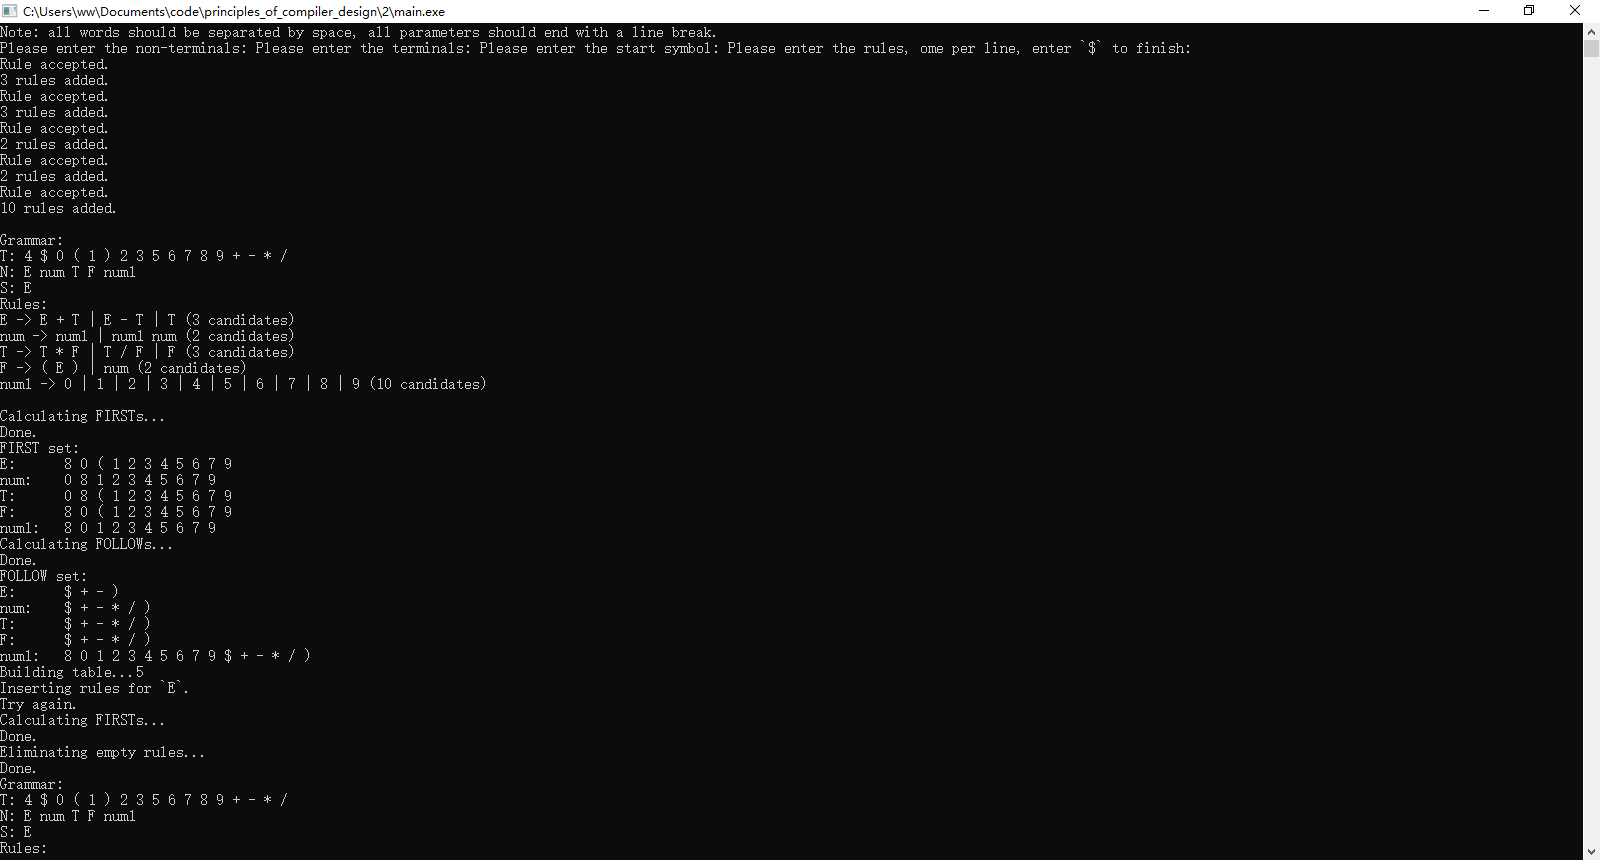
\includegraphics[width=\textwidth]{sample_1}
\begin{lstlisting}
Note: all words should be separated by space, all parameters should end with a line break.
Please enter the non-terminals: Please enter the terminals: Please enter the start symbol: Please enter the rules, ome per line, enter `$` to finish:
Rule accepted.
3 rules added.
Rule accepted.
3 rules added.
Rule accepted.
2 rules added.
Rule accepted.
2 rules added.
Rule accepted.
10 rules added.

Grammar:
T: 4 $ 0 ( 1 ) 2 3 5 6 7 8 9 + - * /
N: E num T F num1
S: E
Rules:
E -> E + T | E - T | T (3 candidates)
num -> num1 | num1 num (2 candidates)
T -> T * F | T / F | F (3 candidates)
F -> ( E ) | num (2 candidates)
num1 -> 0 | 1 | 2 | 3 | 4 | 5 | 6 | 7 | 8 | 9 (10 candidates)

Calculating FIRSTs...
Done.
FIRST set:
E:      8 0 ( 1 2 3 4 5 6 7 9
num:    0 8 1 2 3 4 5 6 7 9
T:      0 8 ( 1 2 3 4 5 6 7 9
F:      8 0 ( 1 2 3 4 5 6 7 9
num1:   8 0 1 2 3 4 5 6 7 9
Calculating FOLLOWs...
Done.
FOLLOW set:
E:      $ + - )
num:    $ + - * / )
T:      $ + - * / )
F:      $ + - * / )
num1:   8 0 1 2 3 4 5 6 7 9 $ + - * / )
Building table...5
Inserting rules for `E`.
Try again.
Calculating FIRSTs...
Done.
Eliminating empty rules...
Done.
Grammar:
T: 4 $ 0 ( 1 ) 2 3 5 6 7 8 9 + - * /
N: E num T F num1
S: E
Rules:
E -> E + T | E - T | T (3 candidates)
num -> num1 | num1 num (2 candidates)
T -> T * F | T / F | F (3 candidates)
F -> ( E ) | num (2 candidates)
num1 -> 0 | 1 | 2 | 3 | 4 | 5 | 6 | 7 | 8 | 9 (10 candidates)

Eliminating all recursions...
Done.
Grammar:
T: 4 $ 0 ( 1 ) 2 3 5 6 7 8 9 + - * /
N: E num T F num1 E' T'
S: E
Rules:
E -> T E' (1 candidates)
num -> num1 | num1 num (2 candidates)
T -> ( E ) T' | num T' (2 candidates)
F -> ( E ) | num (2 candidates)
num1 -> 0 | 1 | 2 | 3 | 4 | 5 | 6 | 7 | 8 | 9 (10 candidates)
E' -> @ | + T E' | - T E' (3 candidates)
T' -> @ | * F T' | / F T' (3 candidates)

Eliminating common prefix...
Done.
Grammar:
T: 4 $ 0 ( 1 ) 2 3 5 6 7 8 9 + - * /
N: E num T F num1 E' num' T'
S: E
Rules:
E -> T E' (1 candidates)
num -> num1 num' (1 candidates)
T -> ( E ) T' | num T' (2 candidates)
F -> ( E ) | num (2 candidates)
num1 -> 8 | 0 | 1 | 2 | 3 | 4 | 5 | 6 | 7 | 9 (10 candidates)
E' -> @ | + T E' | - T E' (3 candidates)
num' -> @ | num (2 candidates)
T' -> @ | * F T' | / F T' (3 candidates)

Calculating FIRSTs...
Done.
FIRST set:
E:      8 0 ( 1 2 3 4 5 6 7 9
num:    0 8 1 2 3 4 5 6 7 9
T:      0 8 ( 1 2 3 4 5 6 7 9
F:      8 0 ( 1 2 3 4 5 6 7 9
num1:   8 0 1 2 3 4 5 6 7 9
E':     @ + -
num':   8 0 @ 1 2 3 4 5 6 7 9
T':     @ * /
Calculating FOLLOWs...
Done.
FOLLOW set:
E:      $ )
num:    * / + - $ )
T:      + - $ )
F:      * / + - $ )
num1:   0 8 1 2 3 4 5 6 7 9 * / + - $ )
E':     $ )
num':   * / + - $ )
T':     + - $ )
Building table...8
Inserting rules for `E`.
Inserting rules for `num`.
Inserting rules for `T`.
Inserting rules for `F`.
Inserting rules for `num1`.
Inserting rules for `E'`.
Inserting rules for `num'`.
Inserting rules for `T'`.
Done.
Analyse table:
Symbol        4        $        0        (        1        )        2        3        5        6        7        8        9        +        -        *        /
    E      TE'    synch      TE'      TE'      TE'    synch      TE'      TE'      TE'      TE'      TE'      TE'      TE'       --       --       --       --
  num num1num'    synch num1num'       -- num1num'    synch num1num' num1num' num1num' num1num' num1num' num1num' num1num'    synch    synch    synch    synch
    T    numT'    synch    numT'    (E)T'    numT'    synch    numT'    numT'    numT'    numT'    numT'    numT'    numT'    synch    synch       --       --
    F      num    synch      num      (E)      num    synch      num      num      num      num      num      num      num    synch    synch    synch    synch
 num1        4    synch        0       --        1    synch        2        3        5        6        7        8        9    synch    synch    synch    synch
   E'       --        @       --       --       --        @       --       --       --       --       --       --       --     +TE'     -TE'       --       --
 num'      num        @      num       --      num        @      num      num      num      num      num      num      num        @        @        @        @
   T'       --        @       --       --       --        @       --       --       --       --       --       --       --        @        @     *FT'     /FT'
Please enter a piece of text to analyse, type `$` to exit:
Analysing `1 + 2`...
  No.                              Stack                                        Input                                     Sentence                   Output
    1                                 $E                                         1+2$                                             E                        E->T E'
    2                               $E'T                                         1+2$                                             TE'                        T->num T'
    3                           $E'T'num                                         1+2$                                             numT'E'                      num->num1 num'
    4                      $E'T'num'num1                                         1+2$                                             num1num'T'E'                     num1->1
    5                         $E'T'num'1                                         1+2$                                             1num'T'E'                    Match
    6                          $E'T'num'                                          +2$                                            1num'T'E'                     num'->@
    7                              $E'T'                                          +2$                                            1T'E'                       T'->@
    8                                $E'                                          +2$                                            1E'                       E'->+ T E'
    9                              $E'T+                                          +2$                                            1+TE'                    Match
   10                               $E'T                                           2$                                           1+TE'                        T->num T'
   11                           $E'T'num                                           2$                                           1+numT'E'                      num->num1 num'
   12                      $E'T'num'num1                                           2$                                           1+num1num'T'E'                     num1->2
   13                         $E'T'num'2                                           2$                                           1+2num'T'E'                    Match
   14                          $E'T'num'                                            $                                          1+2num'T'E'                     num'->@
   15                              $E'T'                                            $                                          1+2T'E'                       T'->@
   16                                $E'                                            $                                          1+2E'                       E'->@
   17                                  $                                            $                                          1+2                 FINISHED
Please enter a piece of text to analyse, type `$` to exit:
Analysing `4 3 + ( 4 + 5 9 ) * 7 8`...
  No.                              Stack                                        Input                                     Sentence                   Output
    1                                 $E                                43+(4+59)*78$                                             E                        E->T E'
    2                               $E'T                                43+(4+59)*78$                                             TE'                        T->num T'
    3                           $E'T'num                                43+(4+59)*78$                                             numT'E'                      num->num1 num'
......
   48                              $E'T'                                            $                                 43+(4+59)*78T'E'                       T'->@
   49                                $E'                                            $                                 43+(4+59)*78E'                       E'->@
   50                                  $                                            $                                 43+(4+59)*78                 FINISHED
Please enter a piece of text to analyse, type `$` to exit:
Analysing `9 6 * ( 6 8 * 0 ) + 2`...
  No.                              Stack                                        Input                                     Sentence                   Output
    1                                 $E                                 96*(68*0)+2$                                             E                        E->T E'
    2                               $E'T                                 96*(68*0)+2$                                             TE'                        T->num T'
    3                           $E'T'num                                 96*(68*0)+2$                                             numT'E'                      num->num1 num'
......
   43                              $E'T'                                            $                                  96*(68*0)+2T'E'                       T'->@
   44                                $E'                                            $                                  96*(68*0)+2E'                       E'->@
   45                                  $                                            $                                  96*(68*0)+2                 FINISHED
Please enter a piece of text to analyse, type `$` to exit:
Analysing `4 3 / ( 9 8 * 9 0 )`...
  No.                              Stack                                        Input                                     Sentence                   Output
    1                                 $E                                  43/(98*90)$                                             E                        E->T E'
    2                               $E'T                                  43/(98*90)$                                             TE'                        T->num T'
    3                           $E'T'num                                  43/(98*90)$                                             numT'E'                      num->num1 num'
......
   39                              $E'T'                                            $                                   43/(98*90)T'E'                       T'->@
   40                                $E'                                            $                                   43/(98*90)E'                       E'->@
   41                                  $                                            $                                   43/(98*90)                 FINISHED
Please enter a piece of text to analyse, type `$` to exit:
Analysing `( 7 9 - 2 3 ) * ( 3 2 + 4 5 )`...
  No.                              Stack                                        Input                                     Sentence                   Output
    1                                 $E                             (79-23)*(32+45)$                                             E                        E->T E'
    2                               $E'T                             (79-23)*(32+45)$                                             TE'                        T->( E ) T'
    3                           $E'T')E(                             (79-23)*(32+45)$                                             (E)T'E'                    Match
......
   58                              $E'T'                                            $                              (79-23)*(32+45)T'E'                       T'->@
   59                                $E'                                            $                              (79-23)*(32+45)E'                       E'->@
   60                                  $                                            $                              (79-23)*(32+45)                 FINISHED
Please enter a piece of text to analyse, type `$` to exit: Press Enter to exit.
    \end{lstlisting}
\subsection{功能测试样例集:$sample\_2.txt$}
程序构建的分析表中含有同步符号$synch$,可进行错误处理
输入文本如下:
\begin{lstlisting}
E T F num num1
( ) 0 1 2 3 4 5 6 7 8 9 + - * /
E
E -> E + T | E - T | T
T -> T * F | T / F | F
F -> ( E ) | num
num -> num1 | num1 num
num1 -> 0 | 1 | 2 | 3 | 4 | 5 | 6 | 7 | 8 | 9
$
1 + 
+ 3
3 + - 4
( 2  + )
2  + 3 )
2  - )
( 2  + 
$
    \end{lstlisting}
将$sample\_2.txt$文件拖拽至$main.exe$文件上,分析语法和其中的$7$个错误样例,程序输出(输出较长,故略去部分) \\
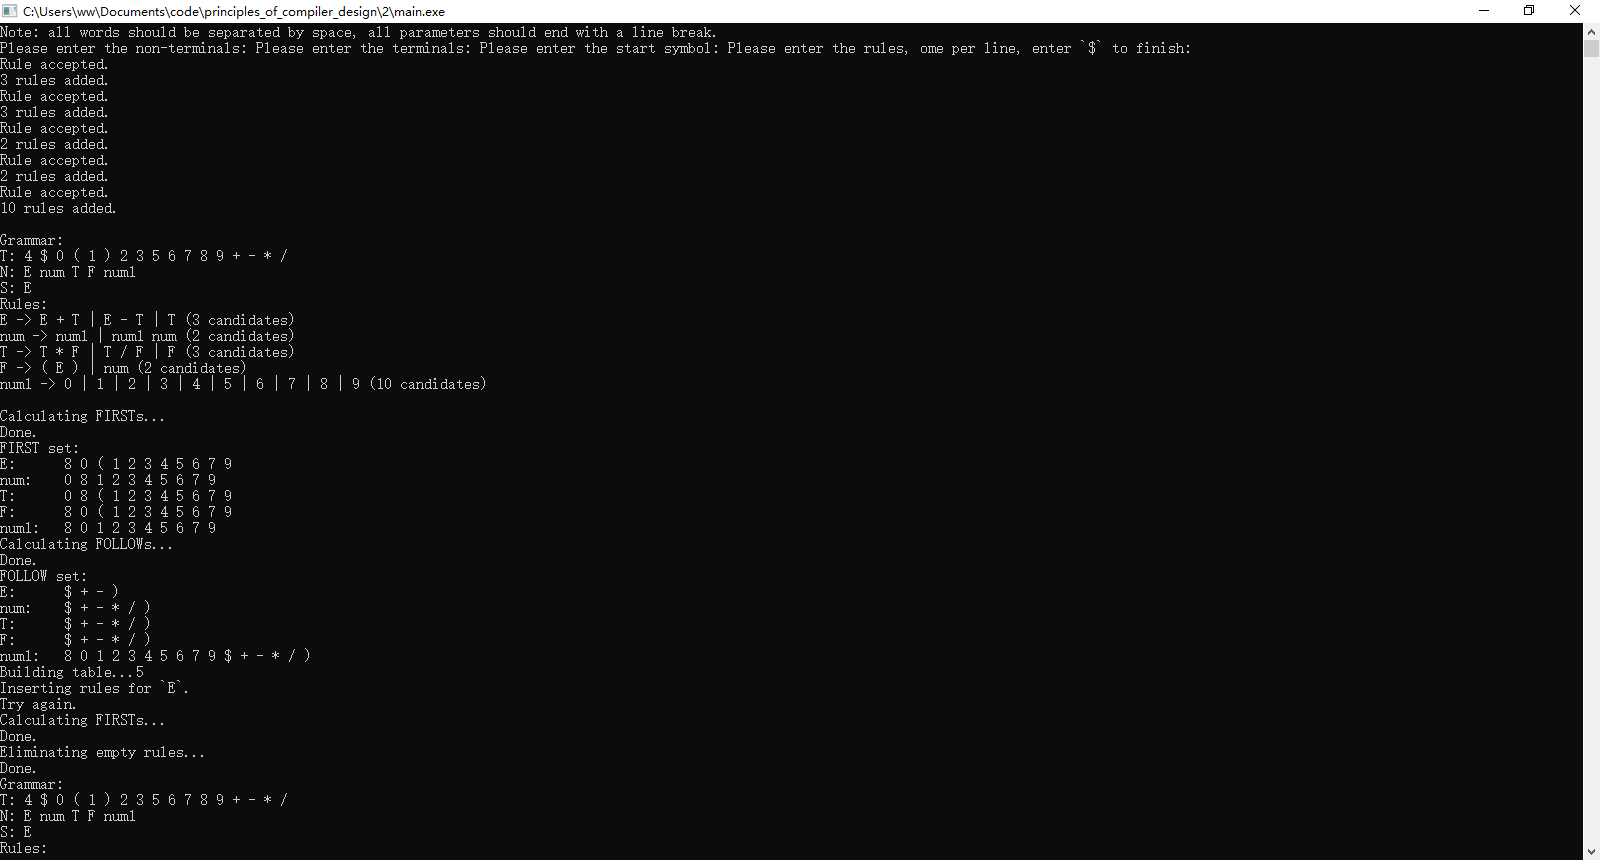
\includegraphics[width=\textwidth]{sample_2}
\begin{lstlisting}
.......
Please enter a piece of text to analyse, type `$` to exit:
Analysing `1 + `...
     No.                    Stack                    Input                      Sentence                                  Output
       1                       $E                      1+$                              E                                       E->T E'
       2                     $E'T                      1+$                              TE'                                       T->num T'
       3                 $E'T'num                      1+$                              numT'E'                                     num->num1 num'
       4            $E'T'num'num1                      1+$                              num1num'T'E'                                    num1->1
       5               $E'T'num'1                      1+$                              1num'T'E'                                   Match
       6                $E'T'num'                       +$                             1num'T'E'                                    num'->@
       7                    $E'T'                       +$                             1T'E'                                      T'->@
       8                      $E'                       +$                             1E'                                      E'->+ T E'
       9                    $E'T+                       +$                             1+TE'                                   Match
      10                     $E'T                        $                            1+TE'       ERROR: pop finished nonterminal `T`
      11                      $E'                        $                            1+E'                                      E'->@
      12                        $                        $                            1+                                FINISHED
Please enter a piece of text to analyse, type `$` to exit:
Analysing `+ 3`...
     No.                    Stack                    Input                      Sentence                                  Output
       1                       $E                      +3$                              E           Error: skip unexpected word `+`.
       2                       $E                       3$                              E                                       E->T E'
       3                     $E'T                       3$                              TE'                                       T->num T'
       4                 $E'T'num                       3$                              numT'E'                                     num->num1 num'
       5            $E'T'num'num1                       3$                              num1num'T'E'                                    num1->3
       6               $E'T'num'3                       3$                              3num'T'E'                                   Match
       7                $E'T'num'                        $                             3num'T'E'                                    num'->@
       8                    $E'T'                        $                             3T'E'                                      T'->@
       9                      $E'                        $                             3E'                                      E'->@
      10                        $                        $                             3                                FINISHED
Please enter a piece of text to analyse, type `$` to exit:
Analysing `3 + - 4`...
     No.                    Stack                    Input                      Sentence                                  Output
       1                       $E                    3+-4$                              E                                       E->T E'
       2                     $E'T                    3+-4$                              TE'                                       T->num T'
       3                 $E'T'num                    3+-4$                              numT'E'                                     num->num1 num'
......
      10                     $E'T                      -4$                            3+TE'       ERROR: pop finished nonterminal `T`
      11                      $E'                      -4$                            3+E'                                      E'->- T E'
......
      19                      $E'                        $                          3+-4E'                                      E'->@
      20                        $                        $                          3+-4                                FINISHED
Please enter a piece of text to analyse, type `$` to exit:
Analysing `( 2  + )`...
     No.                    Stack                    Input                      Sentence                                  Output
       1                       $E                    (2+)$                              E                                       E->T E'
       2                     $E'T                    (2+)$                              TE'                                       T->( E ) T'
......
      13                $E'T')E'T                       )$                           (2+TE')T'E'       ERROR: pop finished nonterminal `T`
      14                 $E'T')E'                       )$                           (2+E')T'E'                                      E'->@
......
      17                      $E'                        $                          (2+)E'                                      E'->@
      18                        $                        $                          (2+)                                FINISHED
Please enter a piece of text to analyse, type `$` to exit:
Analysing `2  + 3 )`...
     No.                    Stack                    Input                      Sentence                                  Output
       1                       $E                    2+3)$                              E                                       E->T E'
       2                     $E'T                    2+3)$                              TE'                                       T->num T'
......
       16                      $E'                       )$                           2+3E'                                      E'->@
      17                        $                       )$                           2+3      FINISHED: with unexpected word(s).
Please enter a piece of text to analyse, type `$` to exit:
Analysing `2  - )`...
     No.                    Stack                    Input                      Sentence                                  Output
       1                       $E                     2-)$                              E                                       E->T E'
       2                     $E'T                     2-)$                              TE'                                       T->num T'
......
      10                     $E'T                       )$                            2-TE'       ERROR: pop finished nonterminal `T`
      11                      $E'                       )$                            2-E'                                      E'->@
      12                        $                       )$                            2-      FINISHED: with unexpected word(s).
Please enter a piece of text to analyse, type `$` to exit:
Analysing `( 2  + `...
     No.                    Stack                    Input                      Sentence                                  Output
       1                       $E                     (2+$                              E                                       E->T E'
       2                     $E'T                     (2+$                              TE'                                       T->( E ) T'
......
      13                $E'T')E'T                        $                           (2+TE')T'E'       ERROR: pop finished nonterminal `T`
      14                 $E'T')E'                        $                           (2+E')T'E'                                      E'->@
      15                   $E'T')                        $                           (2+)T'E'          ERROR: pop finished terminal `)`
      16                    $E'T'                        $                           (2+T'E'                                      T'->@
      17                      $E'                        $                           (2+E'                                      E'->@
      18                        $                        $                           (2+                                FINISHED
Please enter a piece of text to analyse, type `$` to exit: Press Enter to exit.
    \end{lstlisting}
\subsection{功能测试样例集:$sample\_3.txt$}
本程序具有相当的健壮性,可分析相对复杂的句子。
输入文本如下:
\begin{lstlisting}
E T F num num1
( ) 0 1 2 3 4 5 6 7 8 9 + - * /
E
E -> E + T | E - T | T
T -> T * F | T / F | F
F -> ( E ) | num
num -> num1 | num1 num
num1 -> 0 | 1 | 2 | 3 | 4 | 5 | 6 | 7 | 8 | 9
$
1 + ( 3 4 * 7 6 + 9 8 * ( 8 / 3 4 ) ) + ( 2 * ( 3 + ( 4 4 - ( 9 3 / 8 ) ) ) )
$
    \end{lstlisting}
将$sample\_3.txt$文件拖拽至$main.exe$文件上,分析输出(文法与样例$1$一致,略去相关输出,输出较长,略去中间部分): \\
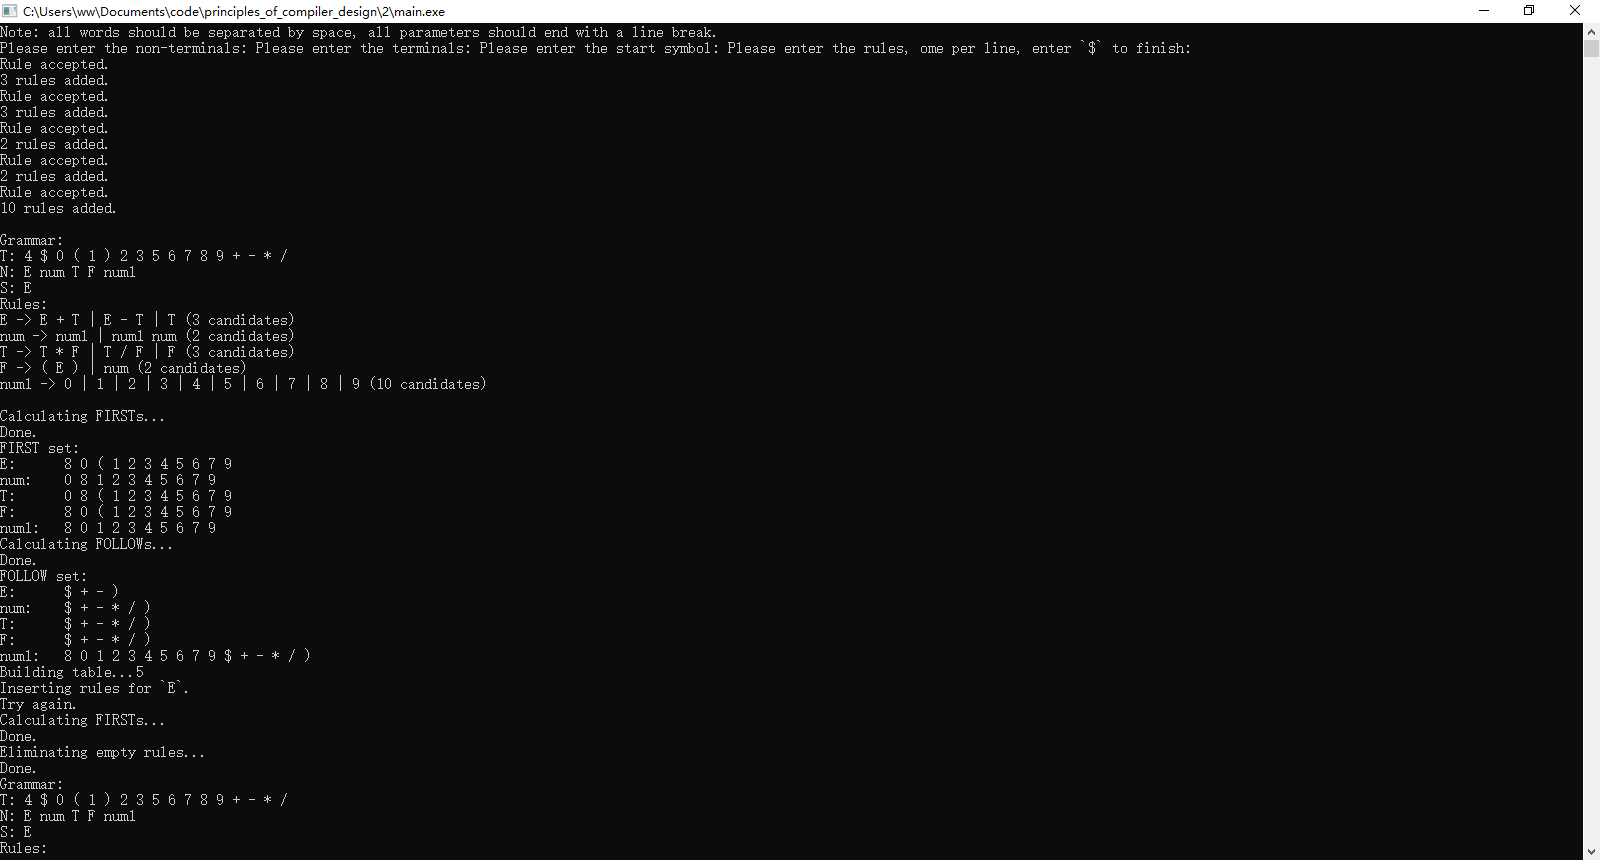
\includegraphics[width=\textwidth]{sample_3}
\begin{lstlisting}
Analysing `1 + ( 3 4 * 7 6 + 9 8 * ( 8 / 3 4 ) ) + ( 2 * ( 3 + ( 4 4 - ( 9 3 / 8 ) ) ) )`...
  No.                              Stack                                        Input                                     Sentence                   Output
    1                                 $E     1+(34*76+98*(8/34))+(2*(3+(44-(93/8))))$                                             E                        E->T E'
    2                               $E'T     1+(34*76+98*(8/34))+(2*(3+(44-(93/8))))$                                             TE'                        T->num T'
    3                           $E'T'num     1+(34*76+98*(8/34))+(2*(3+(44-(93/8))))$                                             numT'E'                      num->num1 num'
    4                      $E'T'num'num1     1+(34*76+98*(8/34))+(2*(3+(44-(93/8))))$                                             num1num'T'E'                     num1->1
    5                         $E'T'num'1     1+(34*76+98*(8/34))+(2*(3+(44-(93/8))))$                                             1num'T'E'                    Match
......
  140                           $E'T')E'                                           )$       1+(34*76+98*(8/34))+(2*(3+(44-(93/8)))E')T'E'                       E'->@
  141                             $E'T')                                           )$       1+(34*76+98*(8/34))+(2*(3+(44-(93/8))))T'E'                    Match
  142                              $E'T'                                            $      1+(34*76+98*(8/34))+(2*(3+(44-(93/8))))T'E'                       T'->@
  143                                $E'                                            $      1+(34*76+98*(8/34))+(2*(3+(44-(93/8))))E'                       E'->@
  144                                  $                                            $      1+(34*76+98*(8/34))+(2*(3+(44-(93/8))))                 FINISHED
Please enter a piece of text to analyse, type `$` to exit: Press Enter to exit.
    \end{lstlisting}
\subsection{功能测试样例集:$sample\_4.txt$}
程序不对用户输入的$LL(1)$文法作任何假设,故本程序可以消除直接和间接左递归,并可检测原文法和改造后的文法是不是$LL(1)$文法,
输入样例$sample\_4.txt$可对此功能进行单元测试。
输入文本如下:
\begin{lstlisting}
Q R S
a b c
R
Q -> R a | a
R -> S b | b
S -> Q c | c
$
acb
$
    \end{lstlisting}
将$sample\_4.txt$文件拖拽至$main.exe$文件上,分析输出: \\
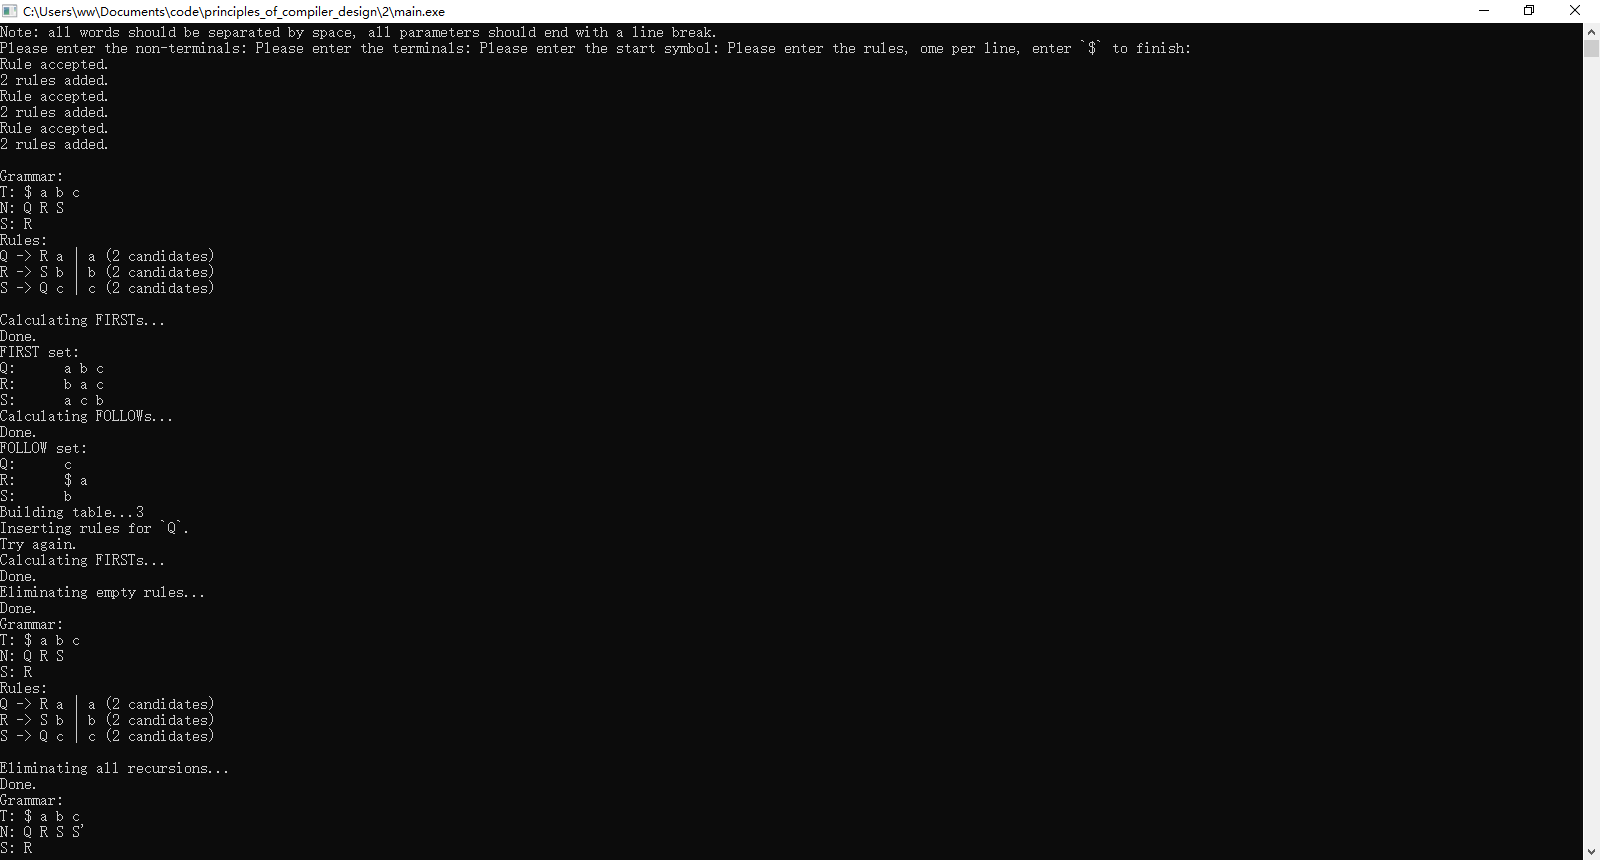
\includegraphics[width=\textwidth]{sample_4}
\begin{lstlisting}
Note: all words should be separated by space, all parameters should end with a line break.
Please enter the non-terminals: Please enter the terminals: Please enter the start symbol: Please enter the rules, ome per line, enter `$` to finish:
Rule accepted.
2 rules added.
Rule accepted.
2 rules added.
Rule accepted.
2 rules added.

Grammar:
T: $ a b c
N: Q R S
S: R
Rules:
Q -> R a | a (2 candidates)
R -> S b | b (2 candidates)
S -> Q c | c (2 candidates)

Calculating FIRSTs...
Done.
FIRST set:
Q:      a b c
R:      b a c
S:      a c b
Calculating FOLLOWs...
Done.
FOLLOW set:
Q:      c
R:      $ a
S:      b
Building table...3
Inserting rules for `Q`.
Try again.
Calculating FIRSTs...
Done.
Eliminating empty rules...
Done.
Grammar:
T: $ a b c
N: Q R S
S: R
Rules:
Q -> R a | a (2 candidates)
R -> S b | b (2 candidates)
S -> Q c | c (2 candidates)

Eliminating all recursions...
Done.
Grammar:
T: $ a b c
N: Q R S S'
S: R
Rules:
Q -> a | S b a | b a (3 candidates)
R -> S b | b (2 candidates)
S -> c S' | a c S' | b a c S' (3 candidates)
S' -> @ | b a c S' (2 candidates)

Eliminating common prefix...
Done.
Grammar:
T: $ a b c
N: Q R S S'
S: R
Rules:
Q -> a | S b a | b a (3 candidates)
R -> S b | b (2 candidates)
S -> c S' | a c S' | b a c S' (3 candidates)
S' -> @ | b a c S' (2 candidates)

Calculating FIRSTs...
Done.
FIRST set:
Q:      a b c
R:      b a c
S:      a c b
S':     @ b
Calculating FOLLOWs...
Done.
FOLLOW set:
Q:
R:      $
S:      b
S':     b
Building table...4
Inserting rules for `Q`.
ERROR: Non-LL(1) grammar detected.
    \end{lstlisting}
\end{document}
